\documentclass[tikz, border=10pt]{standalone}
\usepackage{tikz}
\usepackage[sfdefault]{roboto}
\usepackage[T1]{fontenc}
\usetikzlibrary{shapes.misc, positioning, arrows.meta, fit, calc, backgrounds}

\begin{document}

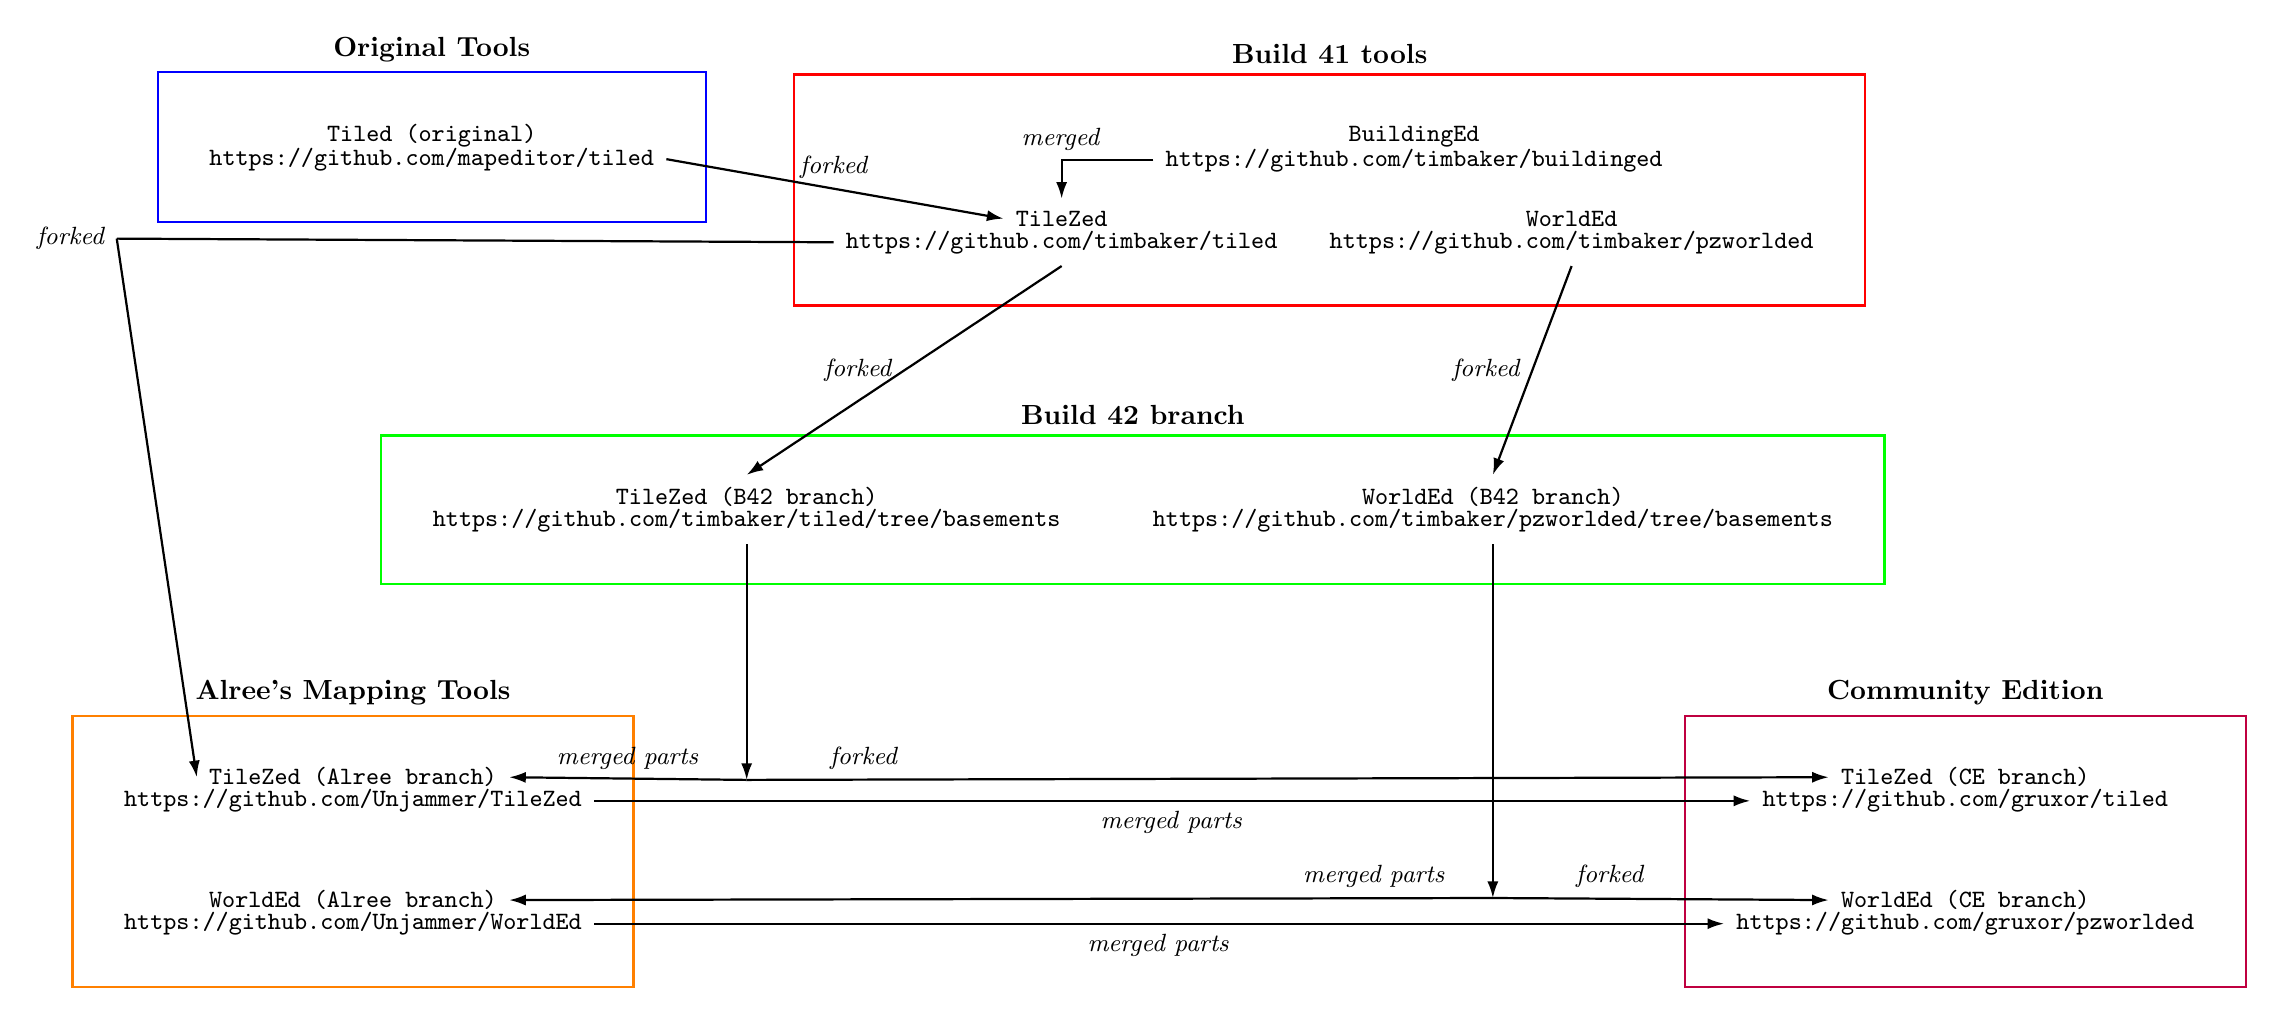
\begin{tikzpicture}[
    node distance=0.3cm,
    box/.style={rectangle, draw, thick, minimum width=5cm, inner sep=0.5cm},
    func/.style={font=\ttfamily\small, inner sep=0.15cm},
    arrow/.style={-{Latex[length=6pt, width=4pt]}, thick},
    line/.style={thick},
]

%% NODES
    % original tools
    \node[func] (ext_tileed) {Tiled (original)};
    \node[func, below of=ext_tileed] (ext_tileed_link) {https://github.com/mapeditor/tiled};

    \begin{scope}[on background layer]
    \node[box, draw=blue!100, fit=(ext_tileed) (ext_tileed_link), label={above:\textbf{Original Tools}}] (external_box) {};
    \end{scope}

    % official tools: B41
    \node[func, below=0.5cm of ext_tileed, xshift=8cm] (tilezed) {TileZed};
    \node[func, below of=tilezed] (tilezed_link) {https://github.com/timbaker/tiled};

    \node[func, right=5cm of tilezed] (worlded) {WorldEd};
    \node[func, below of=worlded] (worlded_link) {https://github.com/timbaker/pzworlded};

    \node[func, above=0.5cm of worlded, xshift=-2cm] (buildinged) {BuildingEd};
    \node[func, below of=buildinged] (buildinged_link) {https://github.com/timbaker/buildinged};
    
    \node[box, draw=red!100, fit=(tilezed) (tilezed_link) (buildinged) (buildinged_link) (worlded) (worlded_link), label={above:\textbf{Build 41 tools}}] (tools_box) {};

    % official tools: B42
    \node[func, below=3cm of tilezed, xshift=-4cm] (tilezed_b42) {TileZed (B42 branch)};
    \node[func, below of=tilezed_b42] (tilezed_b42_link) {https://github.com/timbaker/tiled/tree/basements};

    \node[func, below=3cm of worlded, xshift=-1cm] (worlded_b42) {WorldEd (B42 branch)};
    \node[func, below of=worlded_b42] (worlded_b42_link) {https://github.com/timbaker/pzworlded/tree/basements};

    \node[box, draw=green!100, fit=(tilezed_b42) (tilezed_b42_link) (worlded_b42) (worlded_b42_link), label={above:\textbf{Build 42 branch}}] (b42_box) {};

    % Alree's tools
    \node[func, below=3cm of tilezed_b42, xshift=-5cm] (tilezed_alree) {TileZed (Alree branch)};
    \node[func, below of=tilezed_alree] (tilezed_alree_link) {https://github.com/Unjammer/TileZed};

    \node[func, below=1cm of tilezed_alree] (worlded_alree) {WorldEd (Alree branch)};
    \node[func, below of=worlded_alree] (worlded_alree_link) {https://github.com/Unjammer/WorldEd};

    \node[box, draw=orange!100, fit=(tilezed_alree) (tilezed_alree_link) (worlded_alree) (worlded_alree_link), label={above:\textbf{Alree's Mapping Tools}}] (unofficial_box) {};

    % Community Edition
    \node[func, below=3cm of worlded_b42, xshift=6cm] (tilezed_community) {TileZed (CE branch)};
    \node[func, below of=tilezed_community] (tilezed_community_link) {https://github.com/gruxor/tiled};

    \node[func, below=1cm of tilezed_community] (worlded_community) {WorldEd (CE branch)};
    \node[func, below of=worlded_community] (worlded_community_link) {https://github.com/gruxor/pzworlded};
    
    \node[box, draw=purple!100, fit=(tilezed_community) (tilezed_community_link) (worlded_community) (worlded_community_link), label={above:\textbf{Community Edition}}] (community_box) {};



%% CONNECTIONS
    % original tools -> official tools
    \draw[arrow] (ext_tileed_link.east) -- node[above, font=\small] {\textit{forked}} (tilezed.west);

    % BuildingEd's fusion
    \draw[arrow] (buildinged_link.west) -| node[above, font=\small] {\textit{merged}} (tilezed.north);

    % B41 -> B42
    \draw[arrow] (tilezed_link.south) -- node[left, font=\small] {\textit{forked}} (tilezed_b42.north);
    \draw[arrow] (worlded_link.south) -- node[left, font=\small] {\textit{forked}} (worlded_b42.north);
    % \draw[arrow] (worlded_b42_link.south) |- node[below, font=\small] {\textit{merged parts}} (worlded_alree.east);

    % B41 -> Alree
    \node[func, below=0cm of tilezed, xshift=-12cm] (placeholder) {}; 
    \draw[arrow] (tilezed_link.west) -- (placeholder.north) node[left, font=\small] {\textit{forked}} (placeholder.north) -- (tilezed_alree.west);
    
    % B42 -> intermediate
    \node[func, below=3cm of tilezed_b42] (placeholder_tilezed_b42) {};
    \node[func, below=4.5cm of worlded_b42] (placeholder_worlded_b42) {};

    \draw[arrow] (tilezed_b42_link.south) -- (placeholder_tilezed_b42.south);
    \draw[arrow] (worlded_b42_link.south) -- (placeholder_worlded_b42.south);


    % B42 -> Alree
    \draw[arrow] (placeholder_tilezed_b42.south) node[above, font=\small, xshift=-1.5cm] {\textit{merged parts}}  -- (tilezed_alree.east);
    \draw[arrow] (placeholder_worlded_b42.south) node[above, font=\small, xshift=-1.5cm] {\textit{merged parts}} -- (worlded_alree.east);

    % B42 -> Community Edition
    \draw[arrow] (placeholder_tilezed_b42.south) node[above, font=\small, xshift=1.5cm] {\textit{forked}} -- (tilezed_community.west);
    \draw[arrow] (placeholder_worlded_b42.south) node[above, font=\small, xshift=1.5cm] {\textit{forked}} -- (worlded_community.west);

    % Alree -> Community Edition
    \draw[arrow] (tilezed_alree_link.east) -- node[below, font=\small] {\textit{merged parts}} (tilezed_community_link.west);
    \draw[arrow] (worlded_alree_link.east) -- node[below, font=\small] {\textit{merged parts}} (worlded_community_link.west);

\end{tikzpicture}

\end{document}
